\documentclass{article}
\usepackage[paperwidth=15cm, paperheight=13.0cm, margin = 0cm, top=0.5cm]{geometry}
\usepackage[usenames,dvipsnames]{xcolor}
\usepackage{tikz}
\begin{document}

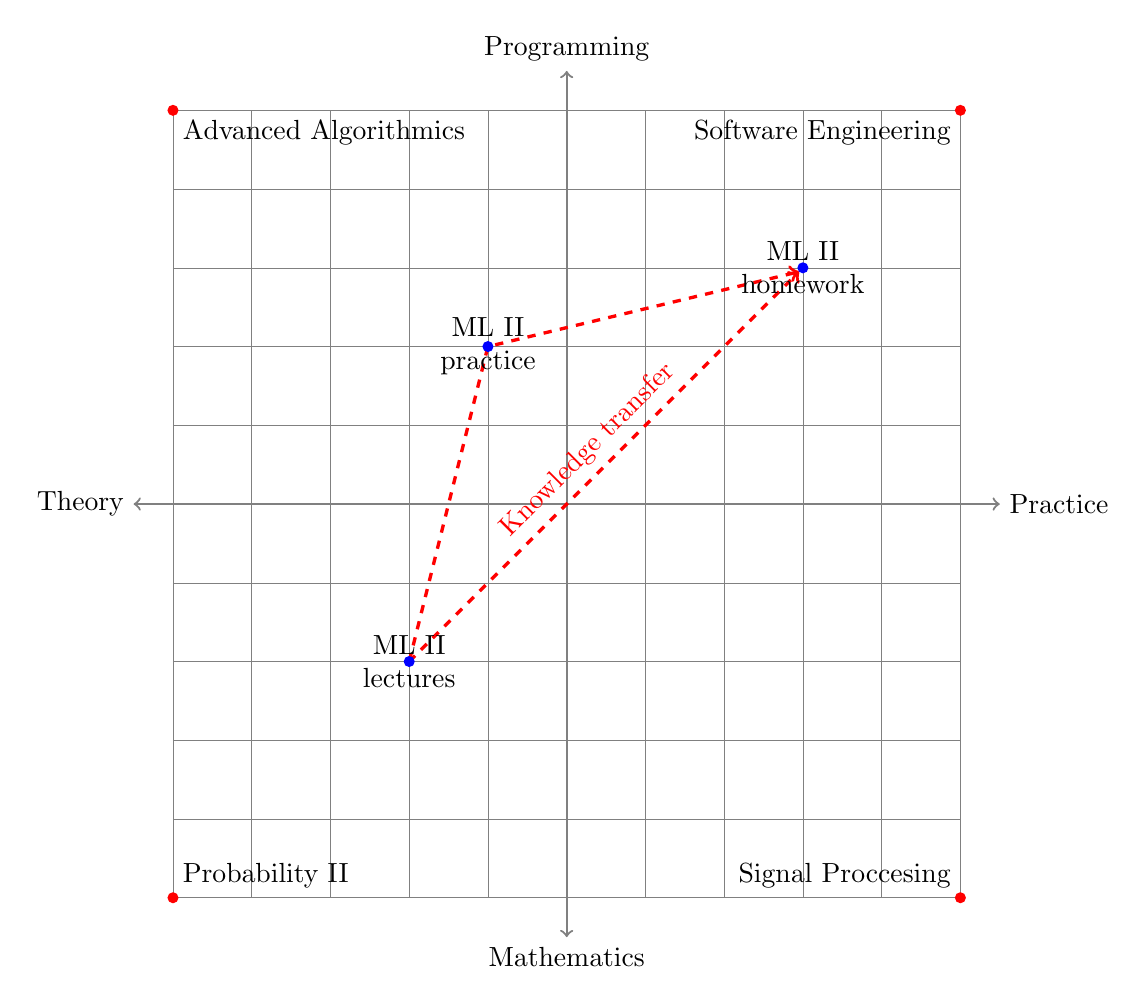
\begin{tikzpicture}
 \draw[gray,thick,<->] (-5.5, 0) -- (5.5, 0);
 \draw[gray,thick,<->] (0, -5.5) -- (0, 5.5);
 \draw[step=1cm,gray,very thin] (-5,-5) grid (5,5);
 \node at (5.5,0)[right]{Practice};
 \node at (-5.5,0)[left]{Theory};
 \node at (0,5.5)[above]{Programming};
 \node at (0,-5.5)[below]{Mathematics};
 
 \fill[red] (-5, -5) circle (2pt) node[anchor=south west, color=black]{Probability II};
 \fill[red] ( 5,  5) circle (2pt) node[anchor=north east, color=black]{Software Engineering};
 \fill[red] ( -5,  5) circle (2pt) node[anchor=north west, color=black]{Advanced Algorithmics};
 \fill[red] ( 5,  -5) circle (2pt) node[anchor=south east, color=black]{Signal Proccesing};

 \draw[->][red,very thick, dashed](-2,-2)--(2.95,2.95) node[midway,above left, sloped, anchor=south]{Knowledge transfer}; 

 \draw[->][red,very thick, dashed](-2,-2)--(-1,2)--(2.95,2.95);

 \fill[blue] ( 3,  3) circle (2pt);
 \node at ( 3,  3)[anchor=center , color=black]{\parbox{2cm}{\begin{center}ML II\\homework\end{center}}};

 \fill[blue] ( -2,  -2) circle (2pt);
 \node at ( -2,  -2)[anchor=center , color=black]{\parbox{2cm}{\begin{center}ML II\\lectures\end{center}}};
 
 \fill[blue] ( -1,  2) circle (2pt);
 \node at ( -1,  2)[anchor=center , color=black]{\parbox{2cm}{\begin{center}ML II\\practice\end{center}}};

 
\end{tikzpicture}
\end{document} 